\chapter{Latent Factor Topic Modelling | Text Clustering}

% \begin{figure}[h]
%    {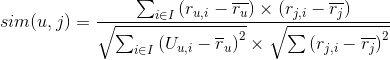
\includegraphics[scale=1]{img/PearsonEqn.png}}
% \end{figure}
Topic Modelling has been a way to comprehend text for the machine learning community. This can be of supervised or unsupervised nature. For the task of this thesis, we have employed the unsupervised version of the topic modelling. A number of simple unsupervised methods can be used for feature selection in text clustering. Some examples of such methods are discussed below.

\section{Document Frequency-based Selection}
The simplest possible method for feature selection in document clustering is that of the use of document frequency to filter out irrelevant features. While the use of inverse document frequencies reduces the importance of such words, this may not alone be sufficient to reduce the noise effects of very frequent words. In other words, words which are too frequent in the corpus can be removed because they are typically common words such as “a”, “an”, “the”, or “of” which are not discriminative from a clustering perspective. Such words are also referred to as stop words. A variety of methods are commonly available in the literature for stop-word removal. Typically commonly available stop word lists of about 300 to 400 words are used for the retrieval process. In addition, words which occur extremely infrequently can also be removed from the collection. This is because such words do not add anything to the similarity computations which are used in most clustering methods. In some cases, such words may be misspellings or typographical errors in documents. Noisy text collections which are derived from the web, blogs or social networks are more likely to contain such terms. We note that some lines of research define document frequency based selection purely on the basis of very infrequent terms, because these terms contribute the least to the similarity calculations. However, it should be emphasized that very frequent words should also be removed, especially if they are not discriminative between clusters. Note that the TF-IDF weighting method can also naturally filter out very common words in a “soft” way. Clearly, the standard set of stop words provide a valid set of words to prune. There are other ways of quantifying the important words directly to the clustering process, which is essential to more aggressive pruning.

\section{Term Strength}
A much more aggressive technique for stop-word removal has been proposed in \cite{Wilbur1992}. The core idea of this approach
is to extend techniques which are used in supervised learning to the unsupervised case. The term strength is essentially used to measure how informative a word is for identifying two related documents. For example, for two related documents x and y, the term strength $s(t)$ of term $t$ is defined in terms of the following probability:
\[
    s(t) = P(t \in y | t \in x)
    \label{eq:probTermStrength} \tag{233}
\]

Clearly, the main issue is how one might define the document x and y as related. One One possibility is to use manual (or user) feedback to define when a pair of documents are related. This is essentially equivalent to utilizing supervision in the feature selection process, and may be practical in situations in which predefined categories of documents are available. On the other hand, it is not practical to manually create related pairs in large collections in a comprehensive way. It is therefore desirable to use an automated and purely unsupervised way to define the concept of when a pair of documents is related. It has been shown in [94] that it is possible to use automated similarity functions such as the cosine function [81] to define the relatedness of document pairs. A pair of documents are defined to be related if their cosine similarity is above a user-defined threshold. In such cases, the term strength s(t) can be defined by randomly sampling a number of pairs of such related documents as follows:
\[
    s(t) = \frac{Number of pairs in which t occurs in both}{Number of pairs in which t occurs in the first of the pair}
    \label{eq:samplingpairs} \tag{234}
\]

Here, the first document of the pair may simply be picked randomly. In order to prune features, the term strength may be compared to the expected strength of a term which is randomly distributed in the training documents with the same frequency. If the term strength of t is not at least two standard deviations greater than that of the random word, then it is removed from the collection.
One advantage of this approach is that it requires no initial supervision or training data for the feature selection, which is a key requirement in the unsupervised scenario. Of course, the approach can also be used for feature selection in either supervised clustering \cite{Bobadilla2013} or categorization\cite{Salakhutdinov2007}, when such training data is indeed available. One observation about this approach to feature selection is that it is particularly suited to similarity-based clustering because the discriminative nature of the underlying features is defined on the basis of similarities in the documents themselves.

\section{Term Contribution}
The concept of term contribution [62] is based on the fact that the results of text clustering are highly dependent on document similarity. Therefore, the contribution of a term can be viewed as its contribution to document similarity. For example, in the case of dot-product based similarity, the similarity between two documents is defined as the dot product of their normalized frequencies. Therefore, the contribution of a term of the similarity of two documents is the product of their normalized frequencies in the two documents. This needs to be summed over all pairs of documents in order to determine the term contribution. As in the previous case, this method requires $O(n^2)$ time for each term, and therefore sampling methods may be required to speed up the contribution. A major criticism of this method is that it tends to favor highly frequent words without regard to the specific discriminative power within a clustering process. In most of these methods, the optimization of term selection is based on some pre-assumed similarity function (e.g., cosine). While this strategy makes these methods unsupervised, there is a concern that the term selection might be biased due to the potential bias of the assumed similarity function. That is, if a different similarity function is assumed, we may end up having different results for term selection. Thus the choice of an appropriate similarity function may be important for these methods.




